\newpage\null\thispagestyle{empty}\newpage
\chapter{Definição do Escopo}
\label{chap:lev_es}

No contexto de DevOps, automação e infraestrutura como código, a ferramenta
proposta por este trabalho, Cupper, propõe auxiliar na extração de configuração
de um ambiente incluso em uma infraestrutura. As configurações extraídas são
transformadas em código em padrões da receita Chef como 
no diagrama da Figura~\ref{fig:cupper_geral}. A
receita gerada é utilizada para qualquer infraestrutura que suporta a
utilização do Chef, como descrito na Seção~\ref{sec:chef}.

\begin{figure}[]
  \centering
  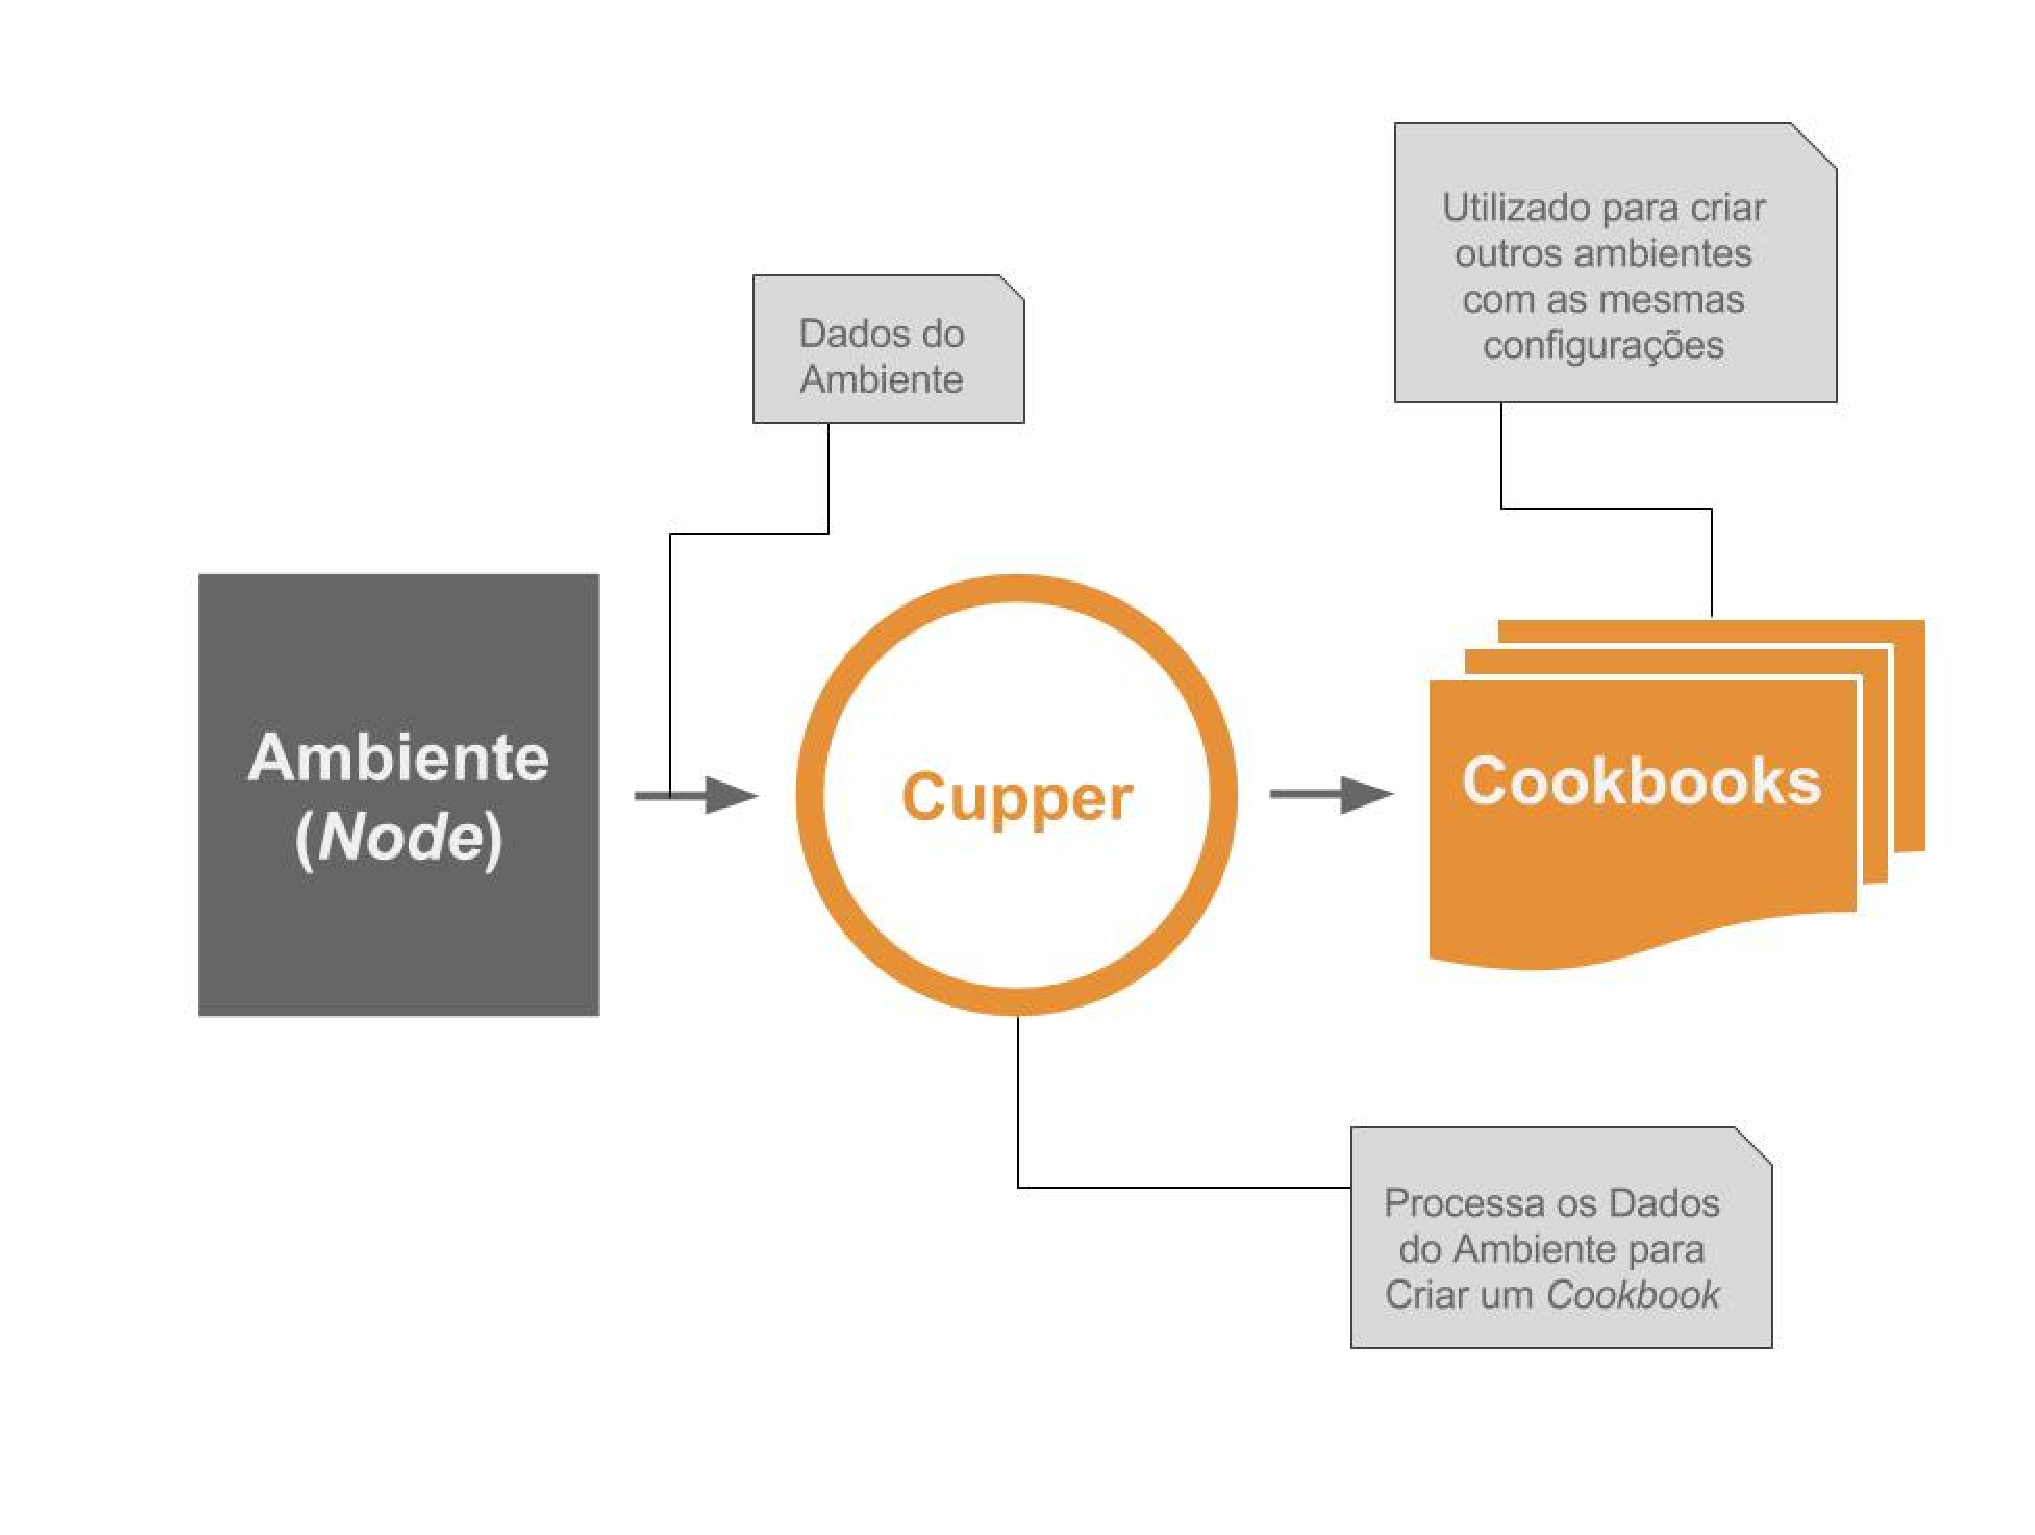
\includegraphics[width=0.8\textwidth]{figuras/cupper_geral.eps}
  \label{fig:cupper_geral}
  \caption{Cupper - Visão geral.}
\end{figure}

Além das dependências de desenvolvimento e de \textit{runtime} por ser uma Gem,
o Cupper tem uma dependência muito
importante que é o Ohai. É requisito desse projeto também implementar
\textit{plugins} para que o Ohai lance informações que por padrão 
não lança.

Nas seções seguinte é mostrado a definição dos itens necessários para
a implementação do Cupper, estando organizados em camadas e seus atributos:

\begin{enumerate}
  \item \textbf{camadas de ambiente}: definição e seleção das camadas de ambiente
    e seus atributos necessários a serem coletados;
  \item \textbf{\textit{cookbook} chef}: definição dos recursos providos pelo \textit{Cookbook} Chef e quais os
    itens necessários para a criação de uma receita mínima;
  \item \textbf{escopo de implementação}: especificação dos itens a serem implementados
    da ferramenta, abordando até qual ponto a ferramenta Cupper pretende alcançar
    até a \textit{release} desse trabalho.
\end{enumerate}

\section{Camadas de Ambiente}
\label{sec:cam-amb}

As camadas apresentam um conjunto de aspectos do sistema e contém as
informações necessárias que definem o comportamento específico para o
estado desejado daquele ambiente. Os atributos de cada camada são variantes
que são consideradas para o implantação de uma aplicação. Sendo assim, as
camadas são dependentes para o nível de compatibilidade da configuração.

As seguintes camadas foram definidas para representar o estado de configuração do
sistema:
\begin{itemize}
  \item \textit{\textbf{Hardware}}: definições físicas onde o sistema foi implantado.
    (Arquitetura, memória, espaço em disco, etc);
  \item \textit{\textbf{Operating System}}: definições do sistema operacional
    implantado. Distribuição, arquitetura, versão, etc;
  \item \textit{\textbf{Application}}: definições das aplicações instaladas.
    (Aplicações instaladas, dependências, etc);
  \item \textit{\textbf{Configuration}}: definições das configurações das
    aplicações. (Especificações de implantação de aplicação, arquivos
    de configuração);
\item \textit{\textbf{Service}}: definições dos serviços \textit{daemon} que estão em
    funcionamento no sistema.
  \item \textit{\textbf{Custom}}: definições criadas especificamente para o
    sistema sem uma forma padrão conhecida.
\end{itemize}

As Tabelas referentes aos atributos relacionados a cada uma dessas camadas se
encontram na Seção~\ref{apc:tabelas} dos apêndices.

\subsection{\textit{Hardware}}
\label{sec:cam-hard}

A camada de \textit{Hardware} contém as definições físicas do sistema.
As informações são referentes as configurações físicas da máquina, como
CPU, arquitetura, memória, espaço em disco, particionamento, etc. O informe desses atributos
são utilizados para a definição da base do ambiente, ou seja, o sistema
operacional e as aplicações podem ter diferentes desempenhos a partir das
configurações de hardware e/ou apresentar comportamentos inesperados no sistema.
Além das aplicações terem seus requisitos mínimos, algumas são desenhadas
para um tipo específico de arquitetura.

A Tabela~\ref{tab:atrhard} mostra diversas informações de hardware possíveis de serem extraídas
do sistema a partir de comandos do sistema operacional e também da ferramenta Ohai, 
dependência prevista para a implementação do Cupper (como descrito na 
Seção~\ref{sec:tec}). Nem todas essas informações serão úteis para a 
implementação, mas nessa Seção fazemos um levantamento geral antes de fazer uma
seleção.
A primeira coluna das Tabelas mostra o atributo em questão; a segunda mostra
a origem do atributo, podendo ser um comando do sistema, ou caminho de um arquivo;
a terceira coluna mostra se o atributo é relevante para a aplicação; a quarta mostra se
esse atributo pode ser conseguido por meio do \textit{Ohai}; a quinta coluna 
diz se é viável implementar o acesso a esse atributo e a ultima coluna
diz se o atributo foi selecionado para ser usado pelo Cupper. 

A camada de hardware será uma das camadas a serem analisadas, e a seleção de 
seus atributos irão seguir os critérios descritos na Seção~\ref{sec:defcritcamada}.

A Tabela~\ref{tab:atrhard} mostra atributos relacionados a CPU, Memória e 
\textit{Moterboard}, e a Tabela~\ref{tab:hdmount} mostra atributos relacionados
a partições, armazenamento, dispositivos PCI, USB e dispositivos de rede.


\subsection{\textit{Operating System}}
\label{sec:cam-os}

A segunda camada de extração de dados é a do Sistema Operacional. 
Cada sistema tem a sua particularidade com relação aos gerenciamento dos 
recursos de hardware e administração de processos. Portanto é necessário a 
construção de uma arquitetura flexível, que contenha os aspectos em comum aos
sistemas operacionais, e modular para que seja possível escalar a utilização 
da ferramenta para mais Sistemas Operacionais.

Inicialmente a ferramenta Cupper irá abordar dois sistemas operacionais, 
ambos baseados em GNU/Linux: Archlinux e Debian.

A Tabela~\ref{tab:so} mostra informações a respeito do Kernel e da distribuição
analisada. Também mostra algumas configurações gerais do sistema, como
configurações de rede.

Por ser específico de cada distribuição linux, não é possível determinar com um
comando qual o gerenciador de pacotes o sistema utiliza. O mesmo acontece para
o sistema de inicialização de serviços e para o módulo de segurança utilizados.
Dessa forma é necessário implementar a captura dessas informações em um plugin 
para o \textit{Ohai}.

\subsection{\textit{Application}}

Essa camada trata das aplicações instaladas no sistema. Aplicações podem ter 
sido instaladas por gerenciadores de pacotes oficiais da distribuição, por
gerenciadores não oficiais, por gerenciadores específicos de módulos para
linguagens e por fim podem ser instalados manualmente. Nessa camada iremos 
suportar somente pacotes instalados por gerenciadores oficiais e por 
gerenciadores específicos de linguagem python e ruby (Pip e RubyGem). Na camada
\textit{Custom} a aplicação irá tentar suportar aplicações instaladas de outras
maneiras.


Nenhum dos atributos dessa camada pode ser extraído pelo \textit{Ohai} por
padrão. Dessa maneira toda a extração desses atributos deverá ser implementada
num plugin para o \textit{Ohai}.

\subsection{\textit{Configuration}}

A análise dessa camada está relacionada às configurações específicas de cada 
aplicação, e do sistema. Dados como especificações de implantação das
aplicações e arquivos de configuração são analisados nessa camada.

Para os arquivos de configuração iremos considerar  o sistema de hierarquia de
sistema de arquivos do linux. Alguns arquivos que não seguem o padrão FHS 
(\textit{Filesystem Hierarchy Standard}, Hierarquia de sistema de arquivos) irão
ser tratados na Seção~\ref{sec:camada-custom} de configurações e instalações \textit{Custom}.

O padrão FHS já prevê alguns sub diretórios para configurações padrão abaixo de
\textit{/etc/} como \textit{/etc/opt, /etc/X11} por exemplo, mas outros diretórios
de arquivos de configuração são importantes, e seguem praticamente o mesmo padrão.
Não serão analisados todos os subdiretórios, só serão analisados os que estiverem
sobre padrão similar ao FHS.

\subsection{\textit{Service}}

Essa camada está relacionada ao gerenciamento de serviços do ambiente.
O gerenciamento de Serviços depende de qual \textit{Init System} é usado pela
distribuição, e em alguns casos, mais de uma abordagem é utilizada por algumas
distribuições.

Existe a maneira de implementar a checagem da presença de um \textit{Init System}
procurando por presença de diretórios e arquivos, mas essa abordagem não é
eficiente. Um exemplo de situação em que isso não funcionaria é a de uma máquina
com Archlinux, ou alguma outra distribuição que siga \textit{rolling release}, e que 
tenha atualizado seu \textit{Init System} por seguir novos padrões da distribuição.
Por não precisar formatar pra atualizar essa nova abordagem, resquícios da abordagem
anterior continuariam presentes na máquina. Isso é comum em distribuições \textit{rolling
release} justamente por sua cultura de não formatar e somente atualizar.

Dessa forma, iremos relacionar os \textit{Init Systems} às distribuições
diretamente levando em conta o \textit{Init System} padrão da distribuição.
A Tabela~\ref{tab:inits-distro} mostra a relação de \textit{Init System} padrão de cada 
distribuição. De qualquer maneira o escopo inicial do projeto prevê
implementação somente para Archlinux e Debian.

\subsection{\textit{Custom}}
\label{sec:camada-custom}

O trabalho referente a essa camada permeia algumas das camadas anteriores, mas
nos pontos em que podem ter procedimentos que não estejam no padrão estabelecido.
Com relação à camada de \textit{Application}, pacotes podem ser instalados por
meio de Makefiles ou scripts customizados que não atualizam o histórico de
pacotes do gerenciador de pacotes. Da mesma maneira, as configurações desses
pacotes podem ser geradas por esses scripts, e colocadas em lugares fora do padrão.
Mesmo considerando aplicações instaladas por gerenciadores de pacotes, vários
arquivos de configuração podem ser instalados em diretórios fora  do padrão FHS.
Dessa maneira, além de \textit{plugins} para o \textit{Ohai}, \textit{plugins}
para o Cupper também devem ser feitos para tratar esses casos especiais.

\section{\textit{Cookbook} Chef}
\label{sec:lev-rec}

Como descrito na Seção~\ref{sec:chef}, o Chef é disposto em vários
componentes. O foco principal do Cupper é a criação de \textit{cookbooks},
sendo assim os recursos levantados são referentes à composição interna
dos \textit{cookbooks}.

Os \textit{cookbooks} contém os seguintes componentes: \textit{attributes, recipes, definitions,
files, libraries, custom resourses, metadata, resources e providers, templates
cookbook versions}~\cite{chefdoc:2016}.

Para o funcionamento de um \textit{cookbook}, com uma estrutura mínima, é necessário que tenha
ao menos um \textit{recipe default} definido. A Figura~\ref{code:tree} mostra essa
estrutura mínima necessária para realizar a configuração do \textit{cookbook app} e a Figura~\ref{code:fulltree} mostra uma estrutura completa.

\renewcommand{\lstlistingname}{Figura}

\noindent\begin{minipage}{.45\textwidth}
  \lstinputlisting[language=Bash, frame=single, label=code:tree, caption="Estrutura mínima de um \textit{cookbook}"]{editaveis/code/minimal_tree}
\end{minipage}\hfill
\noindent\begin{minipage}{.45\textwidth}
  \lstinputlisting[language=Bash, frame=single, label=code:fulltree, caption="Estrutura completa de um \textit{cookbook}"]{editaveis/code/full_tree}
\end{minipage}

\renewcommand{\lstlistingname}{Código}

As Seções seguintes explicam os componentes dos \textit{cookbooks} e quais serão gerados
pelo Cupper.

%\subsection{\textit{Attributes}}
\label{sec:lev-rec-att}

Os \textit{attributes} são os detalhes das especificações do \textit{node}. Definem~\cite{chefdoc:2016}:

\begin{itemize}
  \item o estado atual do \textit{node};
  \item em qual estado o \textit{node} estava após a última execução do \textit{chef-client};
  \item em qual estado o \textit{node} deve alcançar ao final na execução do \textit{chef-client} atual.
\end{itemize}

Os \textit{attributes} são definidos no próprio ambiente através do Ohai, nos \textit{cookbooks},
nos \textit{roles} e \textit{environments}.

Esse atributo será incluido no escopo de implementação. Os \textit{attributes} serão dispostos
de acordo com a coleta dos atributos do ambiente definidos na Seção~\ref{sec:cam-amb}.
Apenas alguns atributos serão inserido como informativo sobre o ambiente, ou seja,
não serão utilizados diretamente no \textit{recipe} do \textit{cookbook}.



\subsection{\textit{Recipes}}
\label{sec:lev-rec-rec}

As \textit{recipes} são as unidades fundamentais para a execução de um \textit{cookbook}. Definem
todas as informações necessárias para configurar o sistema e seguem algumas regras
~\cite{chefdoc:2016}:

\begin{itemize}
  \item Deve ser incluído em um \textit{cookbook};
  \item Deve ser posto em um \textit{run-list} antes de ser usado pelo \textit{chef-client};
  \item É executado na mesma ordem disposta na \textit{run-list};
  \item Pode ser incluído em outro \textit{recipe};
  \item Pode ter dependência de outros \textit{recipe};
  \item Pode marcar um \textit{node} para facilitar a criação de agrupamento.
\end{itemize}

As \textit{recipes} são escritas em Ruby e pode-se utilizar dos recursos providos
pela linguagem. Trata-se de uma coleção desse recursos que são utilizados
para definir as ações das \textit{recipes}. No Código \ref{code:recipe} utiliza-se
três recursos: \textit{package, service} e \textit{template}.

\begin{minipage}{.90\textwidth}
  \lstset{style=shell}
  \lstinputlisting[language=Bash, label=code:recipe, caption=Exemplo de \textit{recipe}. Define a instala{\c{c}}{\~a}o e configura{\c{c}}{\~a}o do \textit{app} Nginx]{editaveis/code/recipe_example.rb}
\end{minipage}

Esse atributo será incluído no escopo de implementação. As \textit{recipes} são os componente chave a
ser gerado pelo Cupper. Nele serão descritos os passos, em sequência lógica de execução,
de todas as configurações. Para cada \textit{cookbook}, será gerado um arquivo de 
\textit{recipe 'default.rb'} contendo todas as informações necessárias para a execução.
A Seção~\ref{sec:cbresource} defini todos os recursos utilizados nas \textit{recipes}.

%
\subsection{\textit{Definitions}}
\label{sec:lev-rec-def}

As \textit{definitions} são um novo tipo de recurso disponível apartir da versão
12.5 do Chef e é recomentado utilizar o \textit{Custom Resource}(Seção \ref{sec:lev-rec-cust})
no lugar de \textit{definitions}~\cite{chefdoc:2016}.

Os \textit{definitions} são comportamento que podem ser reutilizados por outros \textit{recipes}.
São utilizado como recursos padrões de uma receita. No Código \ref{code:definition}
é definido o recurso \textit{host\_porter} com os parametros \textit{port} (valor padrão 4000)
e \textit{hostname} (valor padrão \textit{nil}) que pode ser utilizado em outro
\textit{recipe} com a simples chamada \textit{host\_porter}.

\begin{minipage}{.90\textwidth}
  \lstset{style=shell}
  \lstinputlisting[language=Bash, label=code:definition, caption=Exemplo de \textit{definition}. Adiciona um recurso \textit{host\_porter}.]{editaveis/code/definition_example.rb}
\end{minipage}

Esse atributo não será incluso no escopo de implementação. As \textit{definitions} são
construídas de acordo com as necessidades de cada organização, não sendo
possível prevê-las ou fazer uma \textit{definition} genérica.


\subsection{\textit{Files}}
\label{sec:cbfiles}

Os \textit{Files} são um recurso referente a manipulação de arquivos no ambiente~\cite{chefdoc:2016}.
Pode-se utilizar os seguintes recursos:

\begin{itemize}
  \item \textit{cookbook\_file}: arquivos que são adicionados ao \textit{node} com base
    nos arquivos presentes no diretório \textit{/files} na raiz do \textit{cookbook};
  \item \textit{file}: manipula arquivos que estão presentes no \textit{node};
  \item \textit{remote\_file}: arquivos são adicionado ao \textit{node} a partir de um
    local remoto;
\end{itemize}

Cada recurso \textit{file} é utilizado para um propósito, mas os seus comportamentos
são similares. O Código \ref{code:file} mostra três maneiras diferentes de
inserir o arquivo \textit{eth1-conf} no ambiente.

\begin{minipage}{.90\textwidth}
  \lstset{style=shell}
  \lstinputlisting[language=Bash, label=code:file, caption=Exemplo de \textit{file}. Três modos de inserir o arquivo \textit{eth1-conf}.]{editaveis/code/file_example.rb}
\end{minipage}

Esse atributo será incluído no escopo dos recursos \textit{file} e \textit{cookbook\_file}.
A leitura de um arquivo de configuração ou de implantação de uma aplicação 
é replicado para a pasta \textit{cookbooks/COOKBOOK\_NAME/files/} de mesmo nome.
O \textit{cookbook\_file} será gerado a partir da coleta de arquivos considerado estáticos,
ou seja, o conteúdo não tem variação com relação a nenhum atributo do ambiente,
por exemplo o atributo IP do ambiente.

%\subsection{\textit{Libraries}}

As \textit{libraries} são formas de inserir código Ruby para estender ou definir
uma nova funcionalidade. Semelhante ao que ocorre em \textit{definitions}, entretanto a
capacidade de extensão é maior, sendo possível estender recursos já
existentes~\cite{chefdoc:2016}. Por ser construída em Ruby, todos os
recursos provídos pela linguagem podem ser utilizadas dentro das
\textit{libraries}.

O Código \ref{code:library} mostra a definição para estender um
\textit{recipe} adicionando um método \textit{client} que pode ser utilizado
para facilitar a inserção de dados referente a \textit{ip} e \textit{hostname} de um
\textit{node}

\begin{minipage}{.90\textwidth}
  \lstset{style=shell}
  \lstinputlisting[language=Bash, label=code:library, caption="Exemplo de \textit{libraries}."]{editaveis/code/librarie_example.rb}
\end{minipage}

Em geral, as \textit{libraries} são usadas para definir novas funções que
auxiliam na descrição de rotinas que são mais frequentes durante a
construção de um \textit{recipe} como verificação de arquivos ou serviços.

Esse atributo não será incluido no escopo, pois não é possível definir as \textit{libraries}
necessárias para um contexto desconhecido pelo Cupper.

%
\subsection{\textit{Custom Resource}}
\label{sec:lev-rec-cust}

Adicionado recentemente ao Chef, o \textit{custom resource} é uma forma de criar
novos recursos para os \textit{recipes}. É semelhante as \textit{libraries} e as \textit{definitions},
entretanto é direcionado especificamente para a criação de novos recursos~\cite{chefdoc:2016}.
É uma forma simples de estender o Chef e é implementado dentro de um
\textit{cookbook}.

No Código \ref{code:custom} tem-se a definição de um recurso criado em \textit{cookbooks/app/resources}
com o nome \textit{httpd} e uma propriedade \textit{homepage} com um valor padrão vazio.
Esse recurso é distribuido por todo o \textit{cookbooks} como uma simples chamada
de um recurso Chef como demonstra o Código \ref{code:custom-user}.

\noindent\begin{minipage}{.45\textwidth}
  \lstset{style=shell}
  \lstinputlisting[language=Bash, label=code:custom, caption="Exemplo de declaração de um \textit{custom resource}."]{editaveis/code/custom_example.rb}
\end{minipage}\hfill
\begin{minipage}{.45\textwidth}
  \lstset{style=shell}
  \lstinputlisting[language=Bash, label=code:custom-user, caption="Exemplo de utilização de um \textit{custom resource}."]{editaveis/code/custom_user.rb}
\end{minipage}

Esse atributo não será incluido no escopo, pois a definição dos \textit{custom resource} dependem
da necessidade de cada organização não sendo possível prevê-las.

%
\subsection{\textit{Metadata}}
\label{sec:cbmetadata}

\textit{Metadata} é um arquivo localizado na raiz do \textit{cookbook} como foi monstrado no Código
\ref{code:fulltree}. Nele são definidos informações sobre o \textit{cookbook} como termos de \textit{copyright},
\textit{email} do criador ou da organização, licença, descrição, dependências, etc. São 
todas informações organizacionais e não são obrigatórias.

Esse atributo será incluso no escopo de implementação. Será feito um arquivo padrão de
\textit{metadata} para a representação do \textit{cookbook} gerado pelo Cupper. O usuário deverá
modifica-lo de acordo com as suas necessidades.


\subsection{\textit{Resources e Providers}}
\label{sec:cbresource}

Um \textit{resource} é a definição do passo que deve ser seguido durante o processo
de configuração. Cada \textit{resource} diz ao \textit{chef-client} qual a tarefa a ser executada
como instalar um pacote, criar um arquivo, reiniciar um serviço, etc.
Enquanto o \textit{resource} diz o que deve ser feito, o \textit{provider} diz como deve ser
feito. Por exemplo, o \textit{resource} define \lq\lq instale o pacote A\rq\rq e o \textit{provider} decide
se deve utilizar pacotes deb ou rpm.

Esse atributo será incluso no escopo de implementação. Os \textit{resources} padrão
providos pelo Chef serão utilizados para definir os passos nos arquivos de
\textit{recipes}. Os principais são:

\begin{itemize}
  \item \textit{\textbf{cookbook\_file}}: transfere o arquivo definido em \textit{COOKBOOK\_NAME/files/} para
    uma localização definida (já descrito na Seção \ref{sec:cbfiles});
  \item \textit{\textbf{link}}: usado para criar \textit{links} simbólicos ou real;
  \item \textit{\textbf{package}}: usado para gerenciar pacotes sem a necessidade de especificar a plataforma,
    ou seja, o \textit{provider} irá determinar qual gerenciador de pacote a plataforma utiliza;
  \item \textit{\textbf{service}}: usado para gerenciar serviços da plataforma;
  \item \textit{\textbf{user}}: usado para criar, atualizar, remover e bloquear/desbloquear um usuário do ambiente.
  \item \textit{\textbf{group}}: usado para criar, atualizar, remover um groupo do ambiente.
\end{itemize}

%
\subsection{\textit{Templates}}

Os \textit{templates} são arquivos no formato Embedded Ruby (ERB) e permitem gerar
dinamicamente textos de arquivos estáticos. São muito utilizados em arquivos
de configuração que devem ser modificados de acordo com o ambiente. Os
\textit{templates} são inseridos em \textit{COOKBOOK\_NAME/templates} e deve-se declarar o recurso
\textit{template} nos arquivos de \textit{recipes}.

Esse atributo será incluso no escopo de implementação. A leitura de um arquivo de
configuração ou de implantação de uma aplicação será replicado para a
pasta \textit{cookbook/COOKBOOK\_NAME/templates/} de mesmo nome. Os \textit{templates} serão
gerados apartir da coleta de arquivos considerados din{\^a}mico, ou seja,
o conteúdo contem variáveis que estão relacionado ao atributo do ambiente,
por exemplo o IP do ambiente.


\section{Escopo de Implementação}
\label{sec:escopo}


O Cupper se encaixa na categoria de ferramentas \textit{CLI} (\textit{Command-line Interface})
e como descrito na Seção~\ref{sec:supdev:rubygems}, será construída nos padrões de
RubyGems que permite criar os comandos por meio de arquivos de \textit{script bash}
que serão instalados, por padrão do gerenciado de pacote, no diretório de binários do sistema.
Os comandos serão chamados pelo prefixo \textit{cupper} seguido da funcionalidade e as opções.

%TODO: colocar a estrutura de init do Cupper e mostrar como será a distribuição dos arquivos e diretórios.

Em resumo da Seção~\ref{sec:lev-rec}, os recursos Chef com relação aos \textit{coookbooks} que serão utilizados.

\subsection{Funcionalidades}

\begin{enumerate}
  \item \textbf{Mostrar Ajuda}: imprime no terminal os principais comandos e as opções válidas de
    cada uma;

  \item \textbf{Gerar Cookbook}: extrai as configurações do ambiente e cria o \textit{cookbook} correspondente.
    Esse \textit{cookbook} será inserido no diretório \textit{cookbooks} na raiz do projeto Cupper.
    A Figura~\ref{fig:cupper_geral} mostra o fluxo básico dessa funcionalidade;

  \item \textbf{Mostrar Extrações}: mostra as extrações realizadas pelo Cupper em conjunto com o Ohai,
    ou seja, é a forma intermediária à criação dos \textit{cookbooks} onde serão mostrados os outputs do
    sistema e o reflexo deles no \textit{cookbook} antes da criação em sí;

  \item \textbf{Gerar Projeto Cupper}: gera a estrutura de diretório padrão para o projeto Cupper.
    Um projeto Cupper contém o conjunto de \textit{plugins} do Ohai e Cupper, arquivos de configurações
    específicos do projeto e um conjunto de diretórios onde serão dispostos as configurações
    extraídas e os \textit{cookbooks} gerados do ambiente;

  \item \textbf{Listar \textit{Plugins}}: lista os plugins disponíveis do Ohai, tanto os padrões, já inclusos
    na instalação do Ohai, quanto os customizados pelo Cupper;

\end{enumerate}


